\subsection{Pipeline-Graph}

\begin{center}	
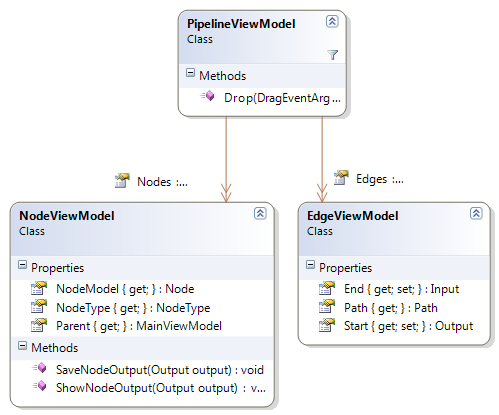
\includegraphics[width=0.5\textwidth]{YuvKA.ViewModel/pipeline.png}
\end{center}
Die Klasse \name{PipelineViewModel} und ihre untergeordneten ViewModels sind für die Darstellung und Manipulation des Pipeline-Graphen zuständig.

\subsubsection{YuvKA.ViewModel.PipelineViewModel}

\begin{verbatim}
public class PipelineViewModel
\end{verbatim}

\paragraph{Beschreibung}~\\
Die \name{PipelineViewModel}-Klasse erzeugt aus dem Graphen des Models passende ViewModels für Knoten und Kanten.

\paragraph{Typmember}
\begin{itemize}

\property{Nodes}
	\begin{verbatim}
	public IList<NodeViewModel> Nodes { get; }
	\end{verbatim}
	Ruft die Menge der Knoten-ViewModels ab.

\method{Edges}
	\begin{verbatim}
	public IEnumerable<EdgeViewModel> Edges { get; }
	\end{verbatim}
	Ruft eine Auflistung von Kanten-ViewModels ab. Der Propertywert wird bei Abruf dynamisch aus der Knotenmenge erzeugt.

\end{itemize}

\subsubsection{YuvKA.ViewModel.NodeViewModel}

\begin{verbatim}
public class NodeViewModel
\end{verbatim}

\paragraph{Beschreibung}~\\
Die \name{NodeViewModel}-Klasse präsentiert die Daten eines \name{Node}-Objekts, sodass sie von der View gebunden werden können.

\paragraph{Typmember}
\begin{itemize}

\property{NodeModel}
	\begin{verbatim}
	public Node NodeModel { get; }
	\end{verbatim}
	Ruft das repräsentierte \name{Node}-Objekt ab.

\property{NodeType}
	\begin{verbatim}
	public NodeType NodeType { get; }
	\end{verbatim}
	Ruft das \name{NodeType}-Objekt ab, das den Typ von \name{NodeModel} repräsentiert.

\method{SaveNodeOutput}
	\begin{verbatim}
	public void SaveNodeOutput(Output output)
	\end{verbatim}
	Rendert das Video des angegebenen Ausgangs und speichert es in einer per \name{SaveFileDialog} ausgewählten Datei.

\method{ShowNodeOutput}
	\begin{verbatim}
	public void ShowNodeOutput(Output output)
	\end{verbatim}
	Öffnet für den angegebenen Ausgang ein neues \name{VideoOutputViewModel}.

\end{itemize}

\subsubsection{YuvKA.ViewModel.EdgeViewModel}

\begin{verbatim}
public class EdgeViewModel
\end{verbatim}

\paragraph{Beschreibung}~\\
Die \name{EdgeViewModel}-Klasse repräsentiert eine Kante im Pipeline-Graph.

\paragraph{Typmember}
\begin{itemize}

\property{Start, Stop}
	\begin{verbatim}
	public Node.Output Start { get; }
	public Node.Input Stop { get; }
	\end{verbatim}
	Rufen Beginn und Ende der Kante ab oder legen sie fest.

\property{Path}
	\begin{verbatim}
	public Path Path { get; }
	\end{verbatim}
	Ruft eine Bezierkurve ab, die die Kante darstellt.

\end{itemize}
